\subsection{Allievi}
\subsubsection{Panoramica allievi}

\begin{figure}[H]
\centering
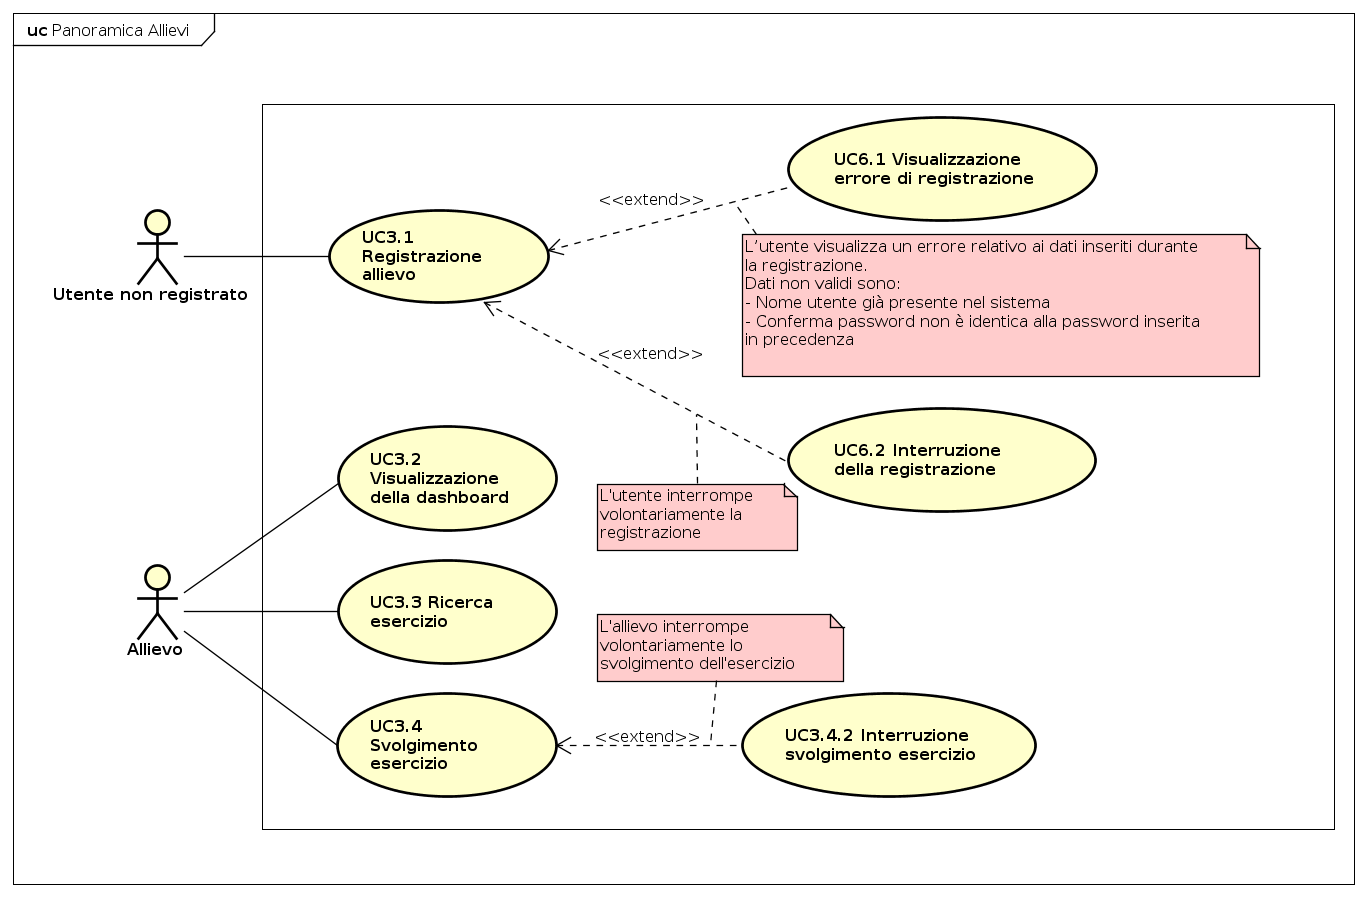
\includegraphics[width=17cm]{img/Panoramica Allievi.png} 
\caption{Panoramica allievi}\label{fig:31}
\end{figure}


\subsubsection{UC 3.2 - Visualizzazione della {dashboard}\ped{G}}
\begin{figure}[H]
\centering
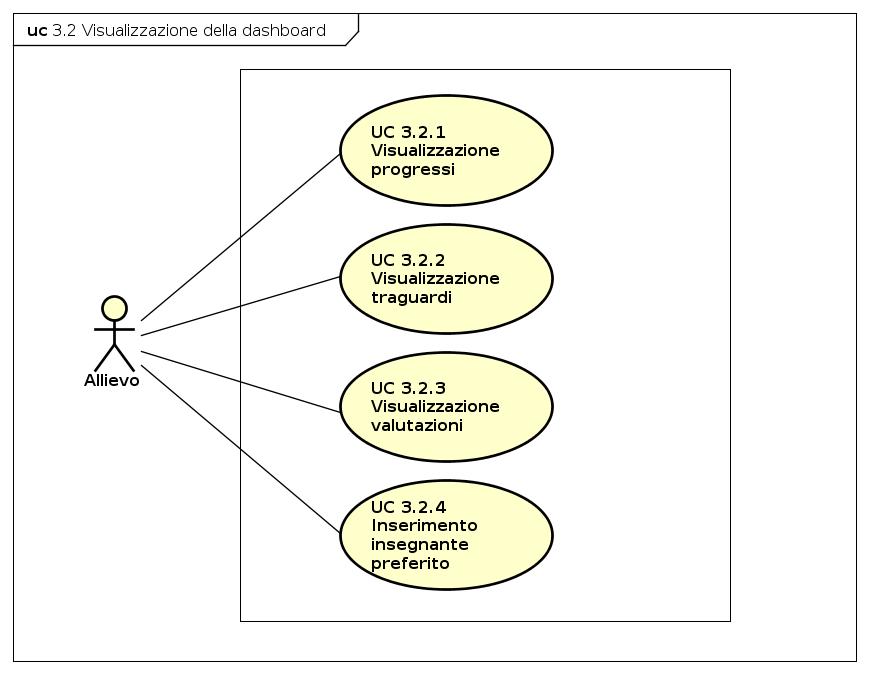
\includegraphics[width=17cm]{img/UC32.png} 
\caption{Caso d'uso 3.2}\label{fig:32}
\end{figure}
\begin{itemize}
\item[•]\textbf{Attori}: Allievo;
\item[•]\textbf{Descrizione}: L'allievo apre la propria {dashboard}\ped{G};
\item[•]\textbf{Precondizione}: L'allievo si è autenticato;
\item[•]\textbf{Postcondizione}: L'allievo ha visualizzato la {dashboard}\ped{G} e può vederne tutte le componenti;
\item[•]\textbf{Flusso degli eventi principale}:
\begin{enumerate}
\item UC 3.2.1 - Visualizzazione progressi;
\item UC 3.2.2 - Visualizzazione traguardi;
\item UC 3.2.3 - Visualizzazione valutazioni;
\item UC 3.2.4 - Inserimento insegnante preferito.
\end{enumerate}
\end{itemize}

\subsubsection{UC 3.2.1 - Visualizzazione progressi}
\begin{itemize}
\item[•]\textbf{Attori}: Allievo;
\item[•]\textbf{Descrizione}: L'allievo visualizza i suoi progressi: numero di esercizi svolti, corretti ed errati;
\item[•]\textbf{Precondizione}: L'allievo ha visualizzato la propria {dashboard}\ped{G};
\item[•]\textbf{Postcondizione}: L'allievo ha visualizzato i propri progressi;
\end{itemize}

\subsubsection{UC 3.2.2 - Visualizzazione traguardi}
\begin{itemize}
\item[•]\textbf{Attori}: Allievo;
\item[•]\textbf{Descrizione}: L'allievo visualizza i traguardi raggiunti;
\item[•]\textbf{Precondizione}: L'allievo ha visualizzato la propria {dashboard}\ped{G};
\item[•]\textbf{Postcondizione}: L'allievo ha visualizzato tutti i traguardi raggiunti;
\end{itemize}

\subsubsection{UC 3.2.3 - Visualizzazione valutazioni}
\begin{itemize}
\item[•]\textbf{Attori}: Allievo;
\item[•]\textbf{Descrizione}: L'allievo visualizza le valutazioni di tutti gli esercizi svolti, sia esercizi assegnati che svolti indipendentemente;
\item[•]\textbf{Precondizione}: L'allievo ha visualizzato la propria {dashboard}\ped{G};
\item[•]\textbf{Postcondizione}: L'allievo ha visualizzato tutte le valutazioni ricevute;
\end{itemize}

\subsubsection{UC 3.2.4 - Inserimento insegnante preferito}
\begin{itemize}
\item[•]\textbf{Attori}: Allievo;
\item[•]\textbf{Descrizione}: L'allievo inserisce il nome utente di un insegnante da prediligere quando riceve la correzione di un esercizio;
\item[•]\textbf{Precondizione}: L'allievo ha visualizzato la propria {dashboard}\ped{G};
\item[•]\textbf{Postcondizione}: L'allievo ha inserito un insegnante preferito;
\end{itemize}

\subsubsection{UC 3.3 - Ricerca esercizio}
\begin{figure}[H]
\centering
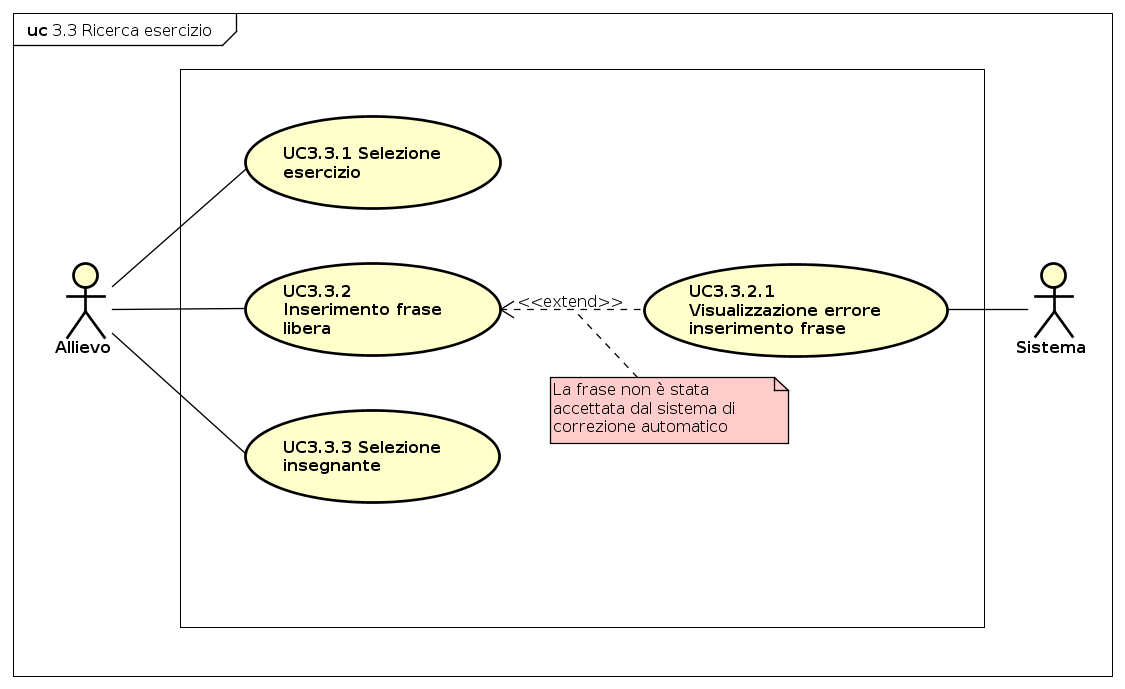
\includegraphics[width=17cm]{img/UC33.png} 
\caption{Caso d'uso 3.3}\label{fig:33}
\end{figure}
\begin{itemize}
\item[•]\textbf{Attori}: Allievo;
\item[•]\textbf{Descrizione}: L'allievo ricerca un esercizio attraverso frasi suggerite dal sistema o attraverso l'inserimento di una frase libera;
\item[•]\textbf{Precondizione}: L'allievo si è autenticato;
\item[•]\textbf{Postcondizione}: L'allievo può navigare una lista di esercizi consigliati o inserire una frase;
\item[•]\textbf{Flusso degli eventi principale}:
\begin{enumerate}
\item UC 3.3.1 - Selezione esercizio;
\item UC 3.3.2 - Inserimento frase libera.
\end{enumerate}
\end{itemize}

\subsubsection{UC 3.3.1 - Selezione esercizio}
\begin{itemize}
\item[•]\textbf{Attori}: Allievo;
\item[•]\textbf{Descrizione}: L'allievo seleziona un esercizio nella lista delle frasi consigliate;
\item[•]\textbf{Precondizione}: L'allievo visualizza una lista di esercizi;
\item[•]\textbf{Postcondizione}: L'allievo ha selezionato un esercizio;
\item[•]\textbf{Flusso degli eventi principale}:
\begin{enumerate}
\item UC 3.3.1.1 - Selezione filtro insegnante.
\end{enumerate}
\end{itemize}

\subsubsection{UC 3.3.1.1 - Selezione filtro insegnante}\begin{figure}[H]
\centering
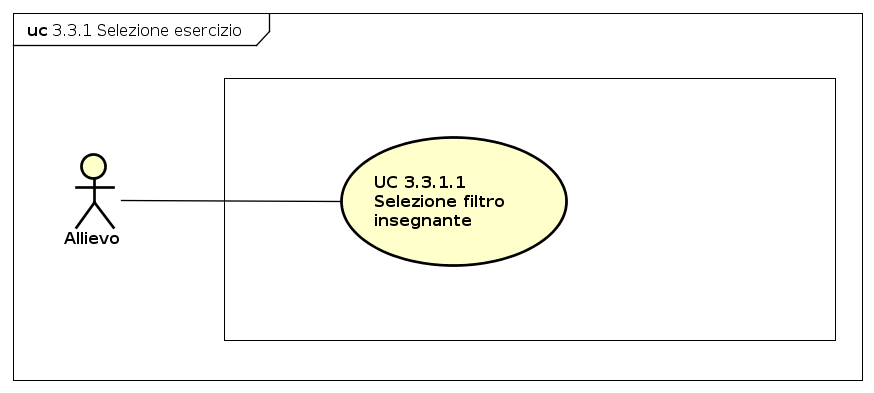
\includegraphics[width=17cm]{img/UC331.png} 
\caption{Caso d'uso 3.3.1}\label{fig:331}
\end{figure}
\begin{itemize}
\item[•]\textbf{Attori}: Allievo;
\item[•]\textbf{Descrizione}: L'allievo seleziona l'insegnante da cui vuole ricevere la correzione dell'esercizio, se nessun insegnante ha predisposto quella frase verrà utilizzato il sistema di correzione automatico. Quando è possibile l'insegnante preferito viene selezionato automaticamente;
\item[•]\textbf{Precondizione}: L'allievo ha selezionato un esercizio;
\item[•]\textbf{Postcondizione}: L'allievo ha selezionato da chi vuole ricevere la correzione;
\end{itemize}

\subsubsection{UC 3.3.2 - Inserimento frase libera}
\begin{itemize}
\item[•]\textbf{Attori}: Allievo;
\item[•]\textbf{Descrizione}: L'allievo inserisce la propria frase in modo da ricevere l'analisi grammaticale di essa;
\item[•]\textbf{Precondizione}: L'allievo vuole inserire una frase;
\item[•]\textbf{Postcondizione}: L'allievo ha correttamente inserito una frase;
\item[•]\textbf{Flusso degli eventi principale}:
\begin{enumerate}
\item UC 3.4.3 - Visualizzazione soluzione.
\end{enumerate}
\item[•]\textbf{Estensioni}:
\begin{enumerate}
\item UC 3.3.2.1 - Visualizzazione errore inserimento frase.
\end{enumerate}
\end{itemize}

\subsubsection{UC 3.3.2.1 - Visualizzazione errore inserimento frase}
\begin{itemize}
\item[•]\textbf{Attori}: Allievo, Libreria di pos-tagging;
\item[•]\textbf{Descrizione}: La frase inserita non è accettata dalla libreria di pos-tagging. L'allievo visualizza un errore e può inserire una nuova frase;
\item[•]\textbf{Precondizione}: L'allievo ha provato ad inserire una frase;
\item[•]\textbf{Postcondizione}: L'allievo ha visualizzato il messaggio di errore e può inserire una nuova frase;
\end{itemize}

\subsubsection{UC 3.4 - Svolgimento esercizio}
\begin{figure}[H]
\centering
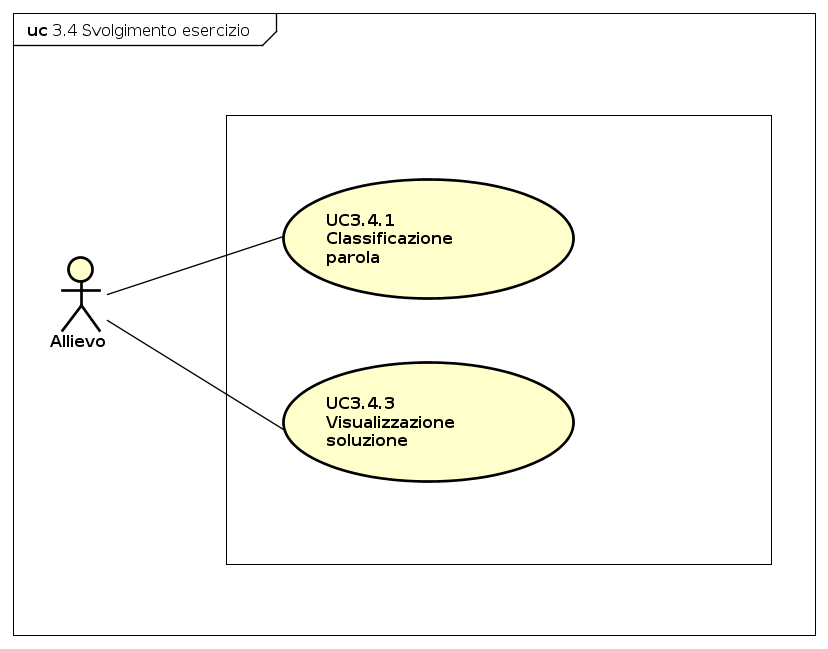
\includegraphics[width=17cm]{img/UC34.png} 
\caption{Caso d'uso 3.4}\label{fig:34}
\end{figure}
\begin{itemize}
\item[•]\textbf{Attori}: Allievo;
\item[•]\textbf{Descrizione}: L'allievo può svolgere l'esercizio scegliendo le classi grammaticali per ciascuna parola da una apposita lista;
\item[•]\textbf{Precondizione}: L'allievo ha selezionato un esercizio;
\item[•]\textbf{Postcondizione}: L'allievo ha svolto un esercizio;
\item[•]\textbf{Flusso degli eventi principale}:
\begin{enumerate}
\item UC 3.4.1 - Classificazione parola;
\item UC 3.4.3 - Visualizzazione soluzione.
\end{enumerate}
\item[•]\textbf{Estensioni}:
\begin{enumerate}
\item UC 3.4.2 - Interruzione svolgimento esercizio.
\end{enumerate}
\end{itemize}

\subsubsection{UC 3.4.1 - Classificazione parola}
\begin{itemize}
\item[•]\textbf{Attori}: Allievo;
\item[•]\textbf{Descrizione}: L'allievo seleziona la classe grammaticale di una parola da una lista predefinita;
\item[•]\textbf{Precondizione}: L'allievo ha iniziato a svolgere un esercizio;
\item[•]\textbf{Postcondizione}: L'allievo ha selezionato la classe grammaticale di una parola;
\end{itemize}

\subsubsection{UC 3.4.2 - Interruzione svolgimento esercizio}
\begin{itemize}
\item[•]\textbf{Attori}: Allievo;
\item[•]\textbf{Descrizione}: L'allievo interrompe l'esercizio, scartando i dati inseriti fino a quel momento, e ritorna nella sezione di ricerca di un esercizio;
\item[•]\textbf{Precondizione}: L'allievo ha iniziato a svolgere un esercizio;
\item[•]\textbf{Postcondizione}: L'allievo ha interrotto l'esercizio, torna nella sezione di ricerca di un esercizio;
\end{itemize}

\subsubsection{UC 3.4.3 - Visualizzazione soluzione}
\begin{itemize}
\item[•]\textbf{Attori}: Allievo, Libreria di pos-tagging;
\item[•]\textbf{Descrizione}: L'allievo visualizza la correzione secondo l'insegnante selezionato in precedenza. Se era stata inserita una frase libera la correzione viene eseguita dal sistema di correzione automatico;
\item[•]\textbf{Precondizione}: L'allievo ha svolto un esercizio oppure ha inserito una frase libera;
\item[•]\textbf{Postcondizione}: L'allievo ha visualizzato la soluzione dell'esercizio;
\item[•]\textbf{Flusso degli eventi principale}:
\begin{enumerate}
\item UC 3.4.3.1 - Visualizzazione valutazione.
\end{enumerate}
\end{itemize}

\subsubsection{UC 3.4.3.1 - Visualizzazione valutazione esercizio}
\begin{figure}[H]
\centering
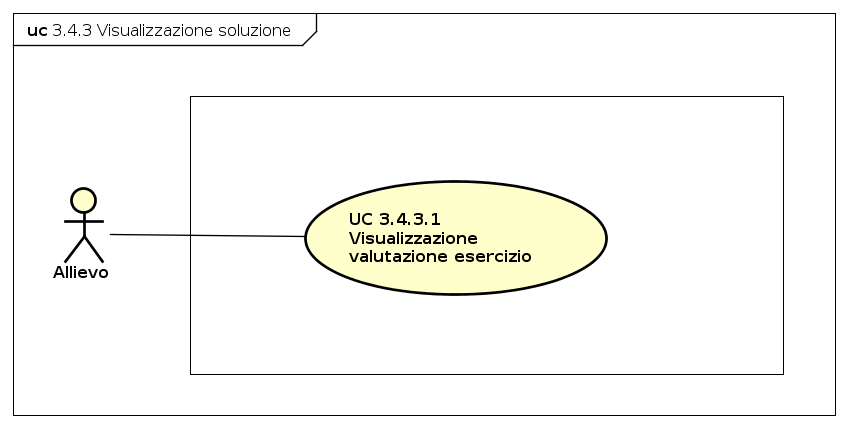
\includegraphics[width=17cm]{img/UC343.png} 
\caption{Caso d'uso 3.4.3}\label{fig:343}
\end{figure}
\begin{itemize}
\item[•]\textbf{Attori}: Allievo;
\item[•]\textbf{Descrizione}: L'allievo riceve una valutazione in base al numero di parole classificate correttamente. Se sono presenti più soluzioni proposte dallo stesso insegnante viene presa la soluzione che porta alla valutazione più alta.
\item[•]\textbf{Precondizione}: L'allievo ha visualizzato la soluzione dell'esercizio svolto;
\item[•]\textbf{Postcondizione}: L'allievo ha visualizzato una valutazione sull'esercizio svolto;
\end{itemize}


